\documentclass[conference]{IEEEtran}
\IEEEoverridecommandlockouts

\usepackage{cite}
\usepackage{amsmath,amssymb,amsfonts}
\usepackage{algorithmic}
\usepackage{graphicx}
\usepackage{textcomp}
\usepackage{xcolor}
\def\BibTeX{{\rm B\kern-.05em{\sc i\kern-.025em b}\kern-.08em
    T\kern-.1667em\lower.7ex\hbox{E}\kern-.125emX}}
\begin{document}

\title{Quantum Computing and The Threat to Cryptographic Systems\\}

\author{
\IEEEauthorblockN{ Aanal Kapadiya} 
\IEEEauthorblockA{
\textit{Department of Computer Science} \\
\textit{University of Tennessee} \\
Knoxville, TN, USA \\
adhanani@vols.utk.edu
} 
\and 
\IEEEauthorblockN{ Alec Riden} 
\IEEEauthorblockA{
\textit{Department of Computer Science} \\
\textit{University of Tennessee} \\
Knoxville, TN, USA \\
ariden1@vols.utk.edu
} 
\and 
\IEEEauthorblockN{ Jarrod Romero Rangel} 
\IEEEauthorblockA{
\textit{Department of Computer Science} \\
\textit{University of Tennessee} \\
Knoxville, TN, USA \\
jromeror@vols.utk.edu
} 
}



\maketitle

\begin{abstract}
    Quantum computing is an emerging field that promises to revolutionize the way we solve complex computational problems. By harnessing the principles of quantum mechanics, quantum computers are capable of performing calculations at speeds far beyond the capabilities of classical computers. This technological advancement holds great potential for applications in fields like optimization, artificial intelligence, and drug discovery. However, while quantum computing offers numerous benefits, it also presents significant challenges, particularly in the realm of cybersecurity. 

    One of the most pressing concerns is the impact quantum computing could have on current encryption systems, which are essential for securing digital communications and data. Classical encryption methods, such as RSA and elliptic curve cryptography (ECC), rely on mathematical problems that are computationally hard to solve. However, quantum algorithms like Shor's algorithm and Grover's algorithm are capable of solving these problems in a fraction of the time it would take a classical computer, thus rendering existing encryption methods vulnerable to quantum attacks. This could have serious implications for the confidentiality and integrity of sensitive information stored and transmitted online.
    
    This paper aims to explore the potential threats posed by quantum computing to modern cryptography, specifically focusing on the vulnerabilities of current encryption systems. It examines the foundational principles of quantum computing and how they could be used to break widely adopted cryptographic algorithms. Furthermore, the paper investigates the ongoing efforts to mitigate these risks, including the development of post-quantum cryptography (PQC), which seeks to create new encryption algorithms that are resistant to quantum attacks, and quantum key distribution (QKD), which offers a way to securely exchange cryptographic keys using quantum channels.
    
    Additionally, this paper reviews the work of organizations like the National Institute of Standards and Technology (NIST), which is actively working to develop standards for quantum-resistant cryptographic methods. While there is significant progress being made in the development of quantum-resistant encryption, there are still several challenges to overcome, such as ensuring the scalability and efficiency of these new systems and integrating them into existing infrastructure.
    
    In conclusion, this paper highlights the urgent need for researchers, policymakers, and industry leaders to work together to address the cybersecurity risks associated with quantum computing. As quantum technologies continue to evolve, it is crucial to develop and implement solutions that will protect our digital infrastructure from potential threats. By examining current efforts and exploring future research directions, this paper contributes to the ongoing discourse on securing digital communications in a quantum-enabled future.
\end{abstract}

\begin{IEEEkeywords}
    Quantum computing, cybersecurity, cryptography, Shor’s algorithm, Grover’s algorithm, post-quantum cryptography, quantum key distribution, NIST, encryption.
\end{IEEEkeywords}
    
\section{Introduction}

Quantum computing is a challenging paradigm that utilizes the principles of quantum mechanics (superposition and entanglement) to accomplish increasingly complex tasks beyond the capabilities of conventional computers. Unlike classical computers, which use binary bits, quantum computers leverage qubits to enable parallel computation at massive scales. Accelerated innovation from industry leaders such as Google and IBM has moved quantum machines from academic experiments to actionable prototypes, marking their potential to revolutionize fields such as cybersecurity.

Cryptography is a fundamental element of digital security, ensuring the privacy, integrity, and authenticity of data in internet-based communication and digital media. Cryptographic methods such as RSA, Elliptic Curve Cryptography (ECC), and other public-key algorithms secure sensitive transactions—from banking to email, to government and military communications. In computer networks, Kuroz and Ross (2021) describe a top-down strategy, as these cryptographic systems underpin various protocols, such as SSL (Secure Sockets Layer), digital signatures, and other high-level exchange protocols. However, these systems, which rely on hard mathematical problems such as integer factorization and discrete logarithms, are vulnerable to attack by quantum computers.

This report aims to evaluate the threats that quantum computing poses to current cryptographic systems. The primary objectives of this report include:
\begin{itemize}
    \item Understanding the principles of quantum computing and how quantum algorithms, such as Shor's and Grover's algorithms, can break and bypass cryptographic security.
    \item Analyzing the vulnerabilities of public-key and symmetric encryption methods in the quantum regime.
    \item Discussing the current efforts toward post-quantum cryptography (PQC) and quantum key distribution (QKD) as potential solutions to these challenges.
    \item Examining the impact of quantum computing on digital infrastructures and providing recommendations for securing these systems in a post-quantum world.
\end{itemize}

As quantum technology advances rapidly, governments, organizations, and individuals are increasingly aware of the potential effects these technologies could have on cybersecurity.

\section{Foundations of Quantum Computing}

Quantum computing is a competitive domain in which the entire principle uses quantum mechanics to process information rather than the conventional method. The difference between classical and quantum computing is that classical computing uses binary bits (0s and 1s) in memory, while quantum computing uses quantum bits, also known as qubits, which essentially offer much greater possibilities due to quantum superposition and entangled states. These highly relevant parameters can maintain cryptographic security, since quantum algorithms will solve particular problems that classical systems cannot \cite{Kurose2021}.

\subsection{Quantum Bits (Qubits) and Superposition}

A classical data processing bit can only be 0 or 1, while qubits are capable of superposition—a quantum phenomenon that allows a particle to be present in both states. The classical bit is present in a defined position, either 0 or 1; on the other hand, a qubit is present in both states at the same time. As more qubits are seen jointly, they exponentially increase the computational power \cite{Nielsen2010}. 

Another main feature of qubits is the incidence of adding two or more qubits with such an entangled correlation, which will immediately inform the other quantum state upon knowing a quantum state, regardless of spatial distance. By promoting more efficient information processing, entanglement allows quantum algorithms to achieve exponential speedups for certain problems\cite{Preskill2018}. Thus, Kurose and Ross \cite{Kurose2021} claim that quantum computing applications may prove advantageous in areas requiring intensive parallel calculations, such as cryptography or network security.

\begin{figure}[htbp]
\centerline{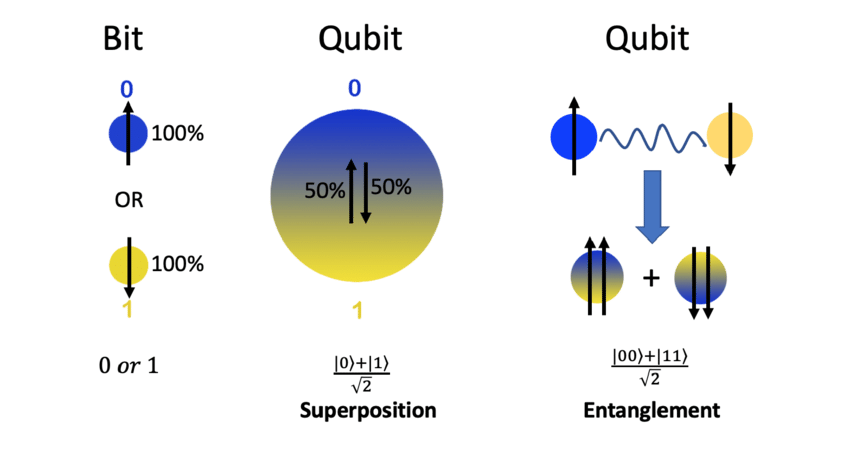
\includegraphics[width=0.5\textwidth]{qubit.png}}
\caption{Illustration of a bit and qubit. (Left) A bit can take a value of '0' or '1' with 100\% probability. (Middle) A qubit can be in a state of $|0\rangle$ or $|1\rangle$ or in a superposition state of both $|0\rangle$ and $|1\rangle$. Here, a qubit is illustrated in a superposition state, composed of 50\% $|0\rangle$ and 50\% $|1\rangle$. (Right) Illustration of two qubits in an entangled state. The properties of the two qubits in an entangled state are linked to each other such that by measuring one of them, the other qubit will be revealed, even when they are at physically large separations.}
\label{figure1}
 \end{figure}
    
As shown in Figure 1 ,a classical bit can only be in a state of 0 or 1, while a qubit can exist in superposition \cite{unknown}.
    

\subsection{Quantum Algorithms Relevant to Cybersecurity}

Most quantum algorithms pose a threat to existing cryptographic techniques, solving complicated mathematical problems much faster than any previous algorithms. Among the most relevant quantum algorithms in the realm of cybersecurity are the following:

\subsubsection{Shor’s Algorithm}

Discovered by Peter Shor and demonstrated in 1994, Shor's algorithm poses a major theoretical challenge to RSA encryption, which forms the basis of security in ECC, as well as the public key cryptosystems vulnerable to noise \cite{Shor1994}. The general understanding is that, while integer factorization is impossible with a classical computer, a quantum computer could easily break these encryption schemes in a very short time due to its computational power. Kurose and Ross \cite{Kurose2021} argue that Shor's algorithm now poses a serious threat to the cryptography in use and should be enhanced for post-quantum cryptography.


\subsubsection{Grover’s Algorithm}

Discovered and developed by Lov Grover in 1996, Grover's algorithm accelerates the speed of searching an unsorted database from $O(N)$ to a time complexity of $O(\sqrt{N})$ \cite{Grover1996}. While symmetric ciphers like AES and SHA-2 could withstand a moderate quantum attack when compared with RSA, Grover's algorithm restores security for practical sizes of symmetric systems, leaving those who implement large sizes for a long period very uneasy \cite{Bernstein2009}.

With the sudden emergence of quantum computing, the race for quantum-resistant cryptographic variants has become an intriguing contrast to classical cryptography. The rest of this paper discusses the potential impact of quantum algorithms on cryptography and the possible applications of quantum-resistant solutions.

\section{The Working of Shor’s Algorithm}

\begin{figure}[htbp]
\centering
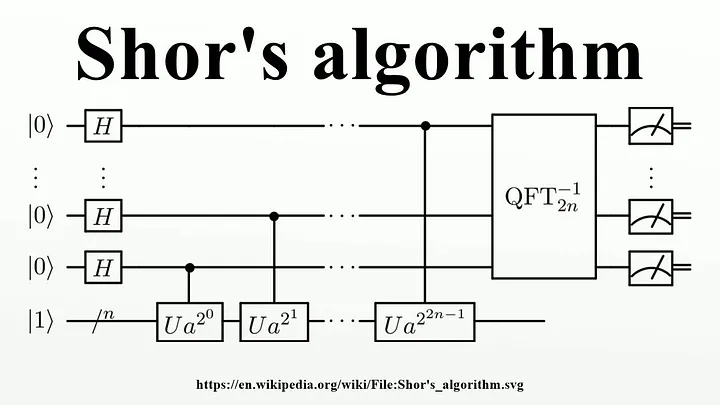
\includegraphics[width=0.50\textwidth]{shors.png}
\caption{Quantum subroutine for order finding in Shor’s algorithm. This circuit is based on Figure 1 in “Circuit for Shor's algorithm using 2n+3 qubits” by Stéphane Beauregard \cite{bender2014shor}.}
\label{fig:shor-circuit}
\end{figure}

As shown in Figure~\ref{fig:shor-circuit}, this quantum subroutine is used in Shor’s algorithm to find the period of a function, a critical step in factoring integers using a quantum computer.\\

To efficiently solve the integer factorization problem, Shor's algorithm uses quantum computing principles, such as quantum parallelism and quantum Fourier transforms (QFTs). The following is a breakdown of the algorithm:    

\begin{itemize}
\item \textbf{Step 1: Period Finding} – The first part of Shor's algorithm involves finding the period \( r \) of a modular exponential function, specifically \( f(x) = a^x \mod N \), where \( a \) is a randomly chosen integer less than \( N \) and \( N \) is the number to be factored. The period \( r \) is crucial because the factorization of \( N \) can be derived from this period \cite{Shor1994}.
    
\item \textbf{Step 2: Quantum Fourier Transform (QFT)} – The period-finding problem is then solved using the quantum Fourier transform, which is a quantum analogue of the discrete Fourier transform. QFT is used to efficiently find the period of the modular function in polynomial time, which is exponentially faster than classical algorithms \cite{Brassard2000}.

\item \textbf{Step 3: Classical Post-Processing} – After obtaining the period \( r \), classical methods such as the Euclidean algorithm are applied to compute the greatest common divisor (GCD) of \( a^{r/2} - 1 \) and \( N \), which yields a nontrivial factor of \( N \).
\end{itemize}

In Shor's algorithm, the speedup is largely due to the quantum Fourier transform. In this form of computation, the process of finding the period can be carried out in polynomial time, which is a huge advantage. It is computationally impossible to factor large numbers, such as those used in RSA encryption, from a classical perspective due to the exponential time and effort involved. However, with Shor’s algorithm, these problems become solvable in polynomial time, threatening the security of classical public-key systems \cite{shor1994}.

As a result cryptographic methods like RSA and elliptic curve cryptography are directly affected, both of which depend on the difficulty of integer factorization or discrete logarithms. The recent advances in the quantum computing field, which have forced a reevaluation of the security of these algorithms, particularly in the context of a post-quantum world \cite{Brassard2000}.

\section{Grover's Algorithm}

\begin{figure}[htbp]Í
\centering

\includegraphics[width=0.50\textwidth]{grover_circuit.png}
\caption{Quantum circuit representation of Grover's algorithm. The circuit includes the Grover oracle which flips the sign of the marked element. Adapted from original work by Fawly~\cite{fawlygrover}.}
\label{fig:grover-circuit}
\end{figure}

In 1996, a method for searching an unsorted database or resolving unstructured search problems called Grover's algorithm. This algorithm offers a quantum speedup in the search process. with a quadratic speedup in brute-force search problems, and this poses a significant impact on symmetric-key cryptography that is similar to Shor's algorithm in the sense that it solves hard problems in polynomial time.

A wide range of problems can be addressed using Grover's algorithm, including cryptographic systems that rely on the difficulty of brute-forcing a particular key in order to identify the key. In particular, the algorithm's influence can be seen very clearly in symmetric encryption schemes such as the Advanced Encryption Standard (AES) and the Secure Hash Algorithm-2 (SHA-2).
\section{The Working of Grover's Algorithm}

Grover's algorithm accelerates the process of searching through an unsorted database of size \( N \), reducing the search time from \( O(N) \) (the classical time complexity) to \( O(\sqrt{N}) \). Here’s a breakdown of the algorithm:

\begin{itemize}
\item \textbf{Superposition and Oracle}- The algorithm begins by preparing a superposition of all possible states. An oracle function is then applied, marking the correct state (the solution to the search problem) by flipping its sign. The quantum state is now a superposition of all possible solutions, with the marked solution having a higher amplitude.

\item \textbf{Amplitude Amplification}- Grover’s algorithm uses an amplitude amplification step to increase the probability of measuring the correct solution. This is done by applying a series of operations that enhance the amplitude of the correct state and reduce the amplitudes of the incorrect ones.

\item \textbf{Iterative Steps}- The algorithm iterates the amplitude amplification step approximately \( \sqrt{N} \) times, where \( N \) is the size of the database. After the iterations, the correct solution will have a significantly higher probability of being measured.

\item \textbf{Quadratic Speedup}- The key insight of Grover’s algorithm is the quadratic speedup: the search for an unsorted database of size \( N \) that would take \( O(N) \) steps classically now takes only \( O(\sqrt{N}) \) steps quantumly.
\end{itemize}
Grover's algorithm presents a threat to symmetric encryption algorithms, like AES, which are used to protect sensitive information in cryptography. For instance, an AES-256 key, which classically requires \( 2^{256} \) steps to brute-force, would only require \( 2^{128} \) quantum operations using this algorithm. It is important to realize that while this is still an infeasible amount of work for quantum computers, the algorithm has less effective security since the complexity is reduced.

Finally, the algorithm suggests that in order to function effectively and economically in post-quantum countries, it may be imperative to increase the key size. Using AES-256, for example, would probably be required to maintain the level of security in a quantum setting as a  classical setting using AES-128.

\section{Current Mitigation Strategies}

\subsection{Post-Quantum Cryptography (PQC)}

\begin{figure}[htbp]
\centering
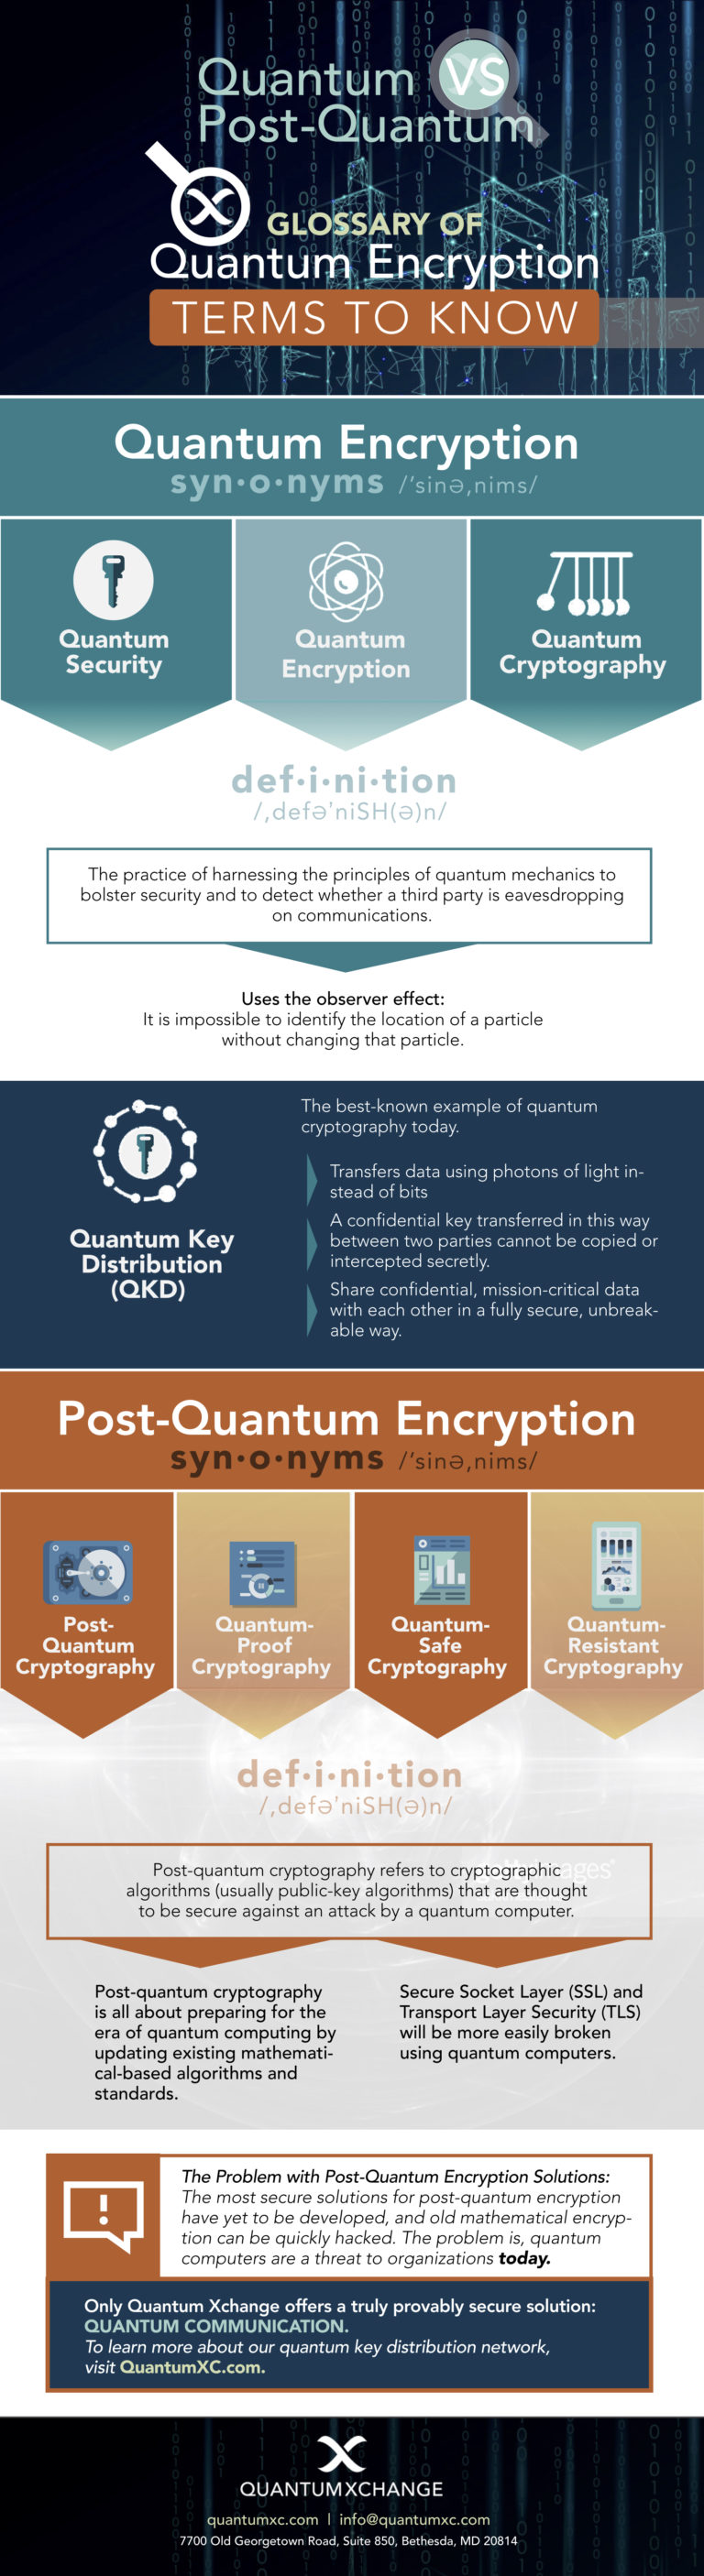
\includegraphics[height=0.8\textheight]{Quantum.jpg}
\caption{Comparison between Quantum Encryption and Post-Quantum Cryptography. Adapted from Quantum Xchange Blog~\cite{quantumxc_infographic}.}
\label{fig:pqc_infographic}
\end{figure}

In the approach of quantum computing, the cryptographic community is working hard to prepare for the inevitable arrival of large-scale quantum computers, which will be a serious threat to the cryptographic systems of the present day. PQC is a technique that is used to develop cryptographic algorithms that are used to create cryptographic systems that are designed to be secure both against classical and quantum computers. This project's aim is to develop encryption methods that are not reliant on mathematical problems that can be efficiently solved by quantum computers. PQC focuses on problems resistant to quantum algorithms, such as lattice-based cryptography, code-based cryptography, and multivariate quadratic equations.

Cryptography using lattices is considered one of the most promising candidates for post-quantum encryption since it relies on the complexity of lattices, which are hard to solve even by quantum computers. Several lattice-based schemes have been proposed for the post-quantum era, including digital signatures, encryption, and homomorphic encryption. In addition to code-based cryptography, multivariate polynomial systems offer alternative routes to quantum-resistant cryptography\cite{Chen2016}.

It is critical to ensure the mathematical security as well as the efficiency of these new algorithms. In order o be used in real-world applications, quantum-safe cryptographic algorithms must be computationally efficient, especially considering that quantum computers may need to be implemented on existing hardware infrastructure first.

\subsection{NIST’s Standardization Efforts}
NIST has taken the lead in standardizing quantum-resistant cryptographic algorithms in order to facilitate the transition from quantum cryptography to post-quantum cryptography. A key objective of NIST's post-quantum cryptography standardization project is to evaluate and select algorithms that will remain secure in the face of quantum attacks while also taking into account factors such as efficiency and practicality. As part of this effort, standardized algorithms were developed in 2016, with the aim of establishing a framework that can be used in the development of future cryptographic systems.

As part of the NIST process, multiple rounds of public evaluation are conducted during which cryptographic researchers from around the world are invited to propose algorithms and provide feedback on existing algorithms. According to NIST, in 2022, finalists and alternative candidates for post-quantum encryption and digital signatures were announced \cite{NIST2022}. with the hope that within the next few years, these algorithms will provide the foundation for developing quantum-resistant cryptographic standards.

As well as being vital to the security of future digital systems, standardization is essential to the global economy as well. In the finance, healthcare, and government industries, cryptographic systems are used to protect sensitive information. NIST's work is focused on ensuring that these systems can withstand quantum computing threats.

\subsection{Quantum Key Distribution (QKD)}

\begin{figure}[htbp]
\centering
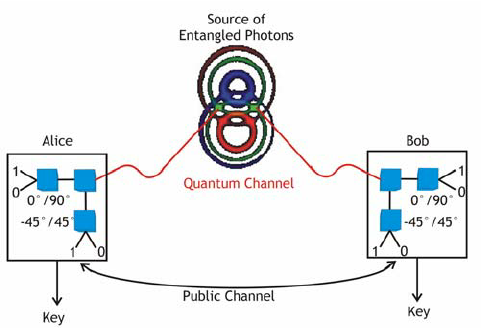
\includegraphics[width=0.5\textwidth]{key.png}
\caption{Quantum Key Distribution (QKD) protocol.}
\label{fig:qkd}
\end{figure}
QKD (Quantum Key Distribution) is another promising approach for securing quantum communications. With quantum key distribution (QKD), cryptographic keys can be securely exchanged between two parties, ensuring that any eavesdropping attempts will be detected. A qubit is used to accomplish this, since it can exist in multiple states simultaneously as a result of superposition. The measurement or intercept of a qubit alters its quantum state, making it possible for the sender and receiver to detect the interference.

In 1984, Bennett and Brassard developed the BB84 protocol, one of the most popular QKD protocols. A basic feature of the BB84 protocol is that it transmits qubits encoded in different polarization states, so the receiver can measure them on the basis of the sender's encoding scheme. When the quantum states of the transmission are disturbed by an eavesdropper, the sender and receiver are alerted to a possible breach \cite{Bennett1992}.

While QKD provides a useful solution for securing communication against quantum adversaries, several practical challenges remain. QKD is currently limited by distance due to photon loss over optical fibers, and scaling the technology will be expensive. In spite of these challenges, quantum communication technologies will continue to advance, making QKD more feasible for secure communication.

\section{Hybrid Cryptographic Models}

Due to the continued evolution of quantum computing, the cryptographic community is exploring interim solutions for bridging the gap between classical and post-quantum cryptography. In order to maintain robust security regardless of quantum adversaries in the future, hybrid cryptographic models offer a practical transitional approach, combining traditional and quantum-resistant algorithms. A quantum-resilient model is especially valuable during the migration period when quantum-resistant standards have not yet been universally adopted or fully tested.

As one example of hybrid encryption, RSA, a classical public-key algorithm, is used in conjunction with Kyber, a post-quantum, lattice-based algorithm. Dual encryption uses both algorithms to encrypt messages. To decrypt the message's plaintext, one must decrypt both encrypted versions. A safety net is provided by the post-quantum layer, since it guarantees that data is still protected even if quantum computers render RSA obsolete. The RSA layer may still provide temporary protection, however, if a newly deployed PQC algorithm exhibits an unforeseen vulnerability.

Additionally, hybrid models help ensure backward compatibility with legacy systems that cannot be upgraded quickly. They facilitate secure communication between systems at various stages of PQC readiness, thereby reducing the risk of premature or inconsistent adoption. There are trade-offs associated with hybrid encryption, however, such as increased bandwidth demands and computational overheads. In order to balance performance with long-term security during this cryptographic transition, strategic planning is essential.

\section{Lattice-Based Cryptography for Post-Quantum Security}

\begin{figure}[htbp]
\centering
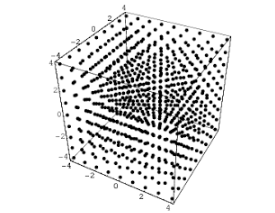
\includegraphics[width=\linewidth]{Lattice.png}
\caption{Overview of Lattice-Based Cryptography. The figure illustrates the concept of lattices as periodic grids of integer vectors, foundational to lattice-based cryptographic schemes.}
\label{fig:lattice_crypto_overview}
\end{figure}

Lattice-based encryption schemes have emerged as one of the most promising approaches in the quest for quantum-resistant cryptography. Unlike traditional systems that rely on factoring large numbers or computing discrete logarithms, lattice-based schemes are grounded in problems related to geometric arrangements of points in multi-dimensional space—specifically, finding the shortest or closest vector in a lattice. These problems are known to be hard for both classical and quantum computers, making them strong candidates for post-quantum cryptography. One widely studied lattice-based system is Learning With Errors (LWE), which involves solving systems of noisy linear equations—a task believed to be resistant even to quantum algorithms \cite{Regev2009}. These mathematical foundations provide strong security guarantees and support advanced features like homomorphic encryption, which allows computations to be performed directly on encrypted data without decryption \cite{Cheng2025}. This makes lattice-based cryptography a secure and versatile solution suitable for applications beyond simple data transmission.

However, despite their theoretical advantages, deploying lattice-based encryption schemes in real-world systems can present several challenges. One such challenge is performance. Compared to traditional algorithms like RSA or ECC, lattice-based schemes often require significantly larger key sizes and ciphertexts, which can increase bandwidth and storage demands \cite{Bos2018}. For example, Kyber, a leading lattice-based algorithm selected in NIST's post-quantum cryptography standardization process, has key sizes that are much larger than those used in RSA, which may pose issues for devices with limited computational power or memory. Additionally, because lattice-based cryptography is relatively new, it lacks the extensive optimization that classical algorithms have undergone over decades. This increases the risk of implementation flaws or side-channel vulnerabilities, which attackers could exploit regardless of the underlying mathematical security.

Another significant challenge in deploying lattice-based encryption lies in the widespread integration of quantum-resistant systems into existing digital infrastructure. Developers and engineers typically deeply embed cryptographic algorithms worldwide in their software, hardware, and communication protocols. Replacing them with quantum-safe alternatives is not a simple plug-and-play operation; it requires extensive testing, validation, and coordination among developers, vendors, and regulatory bodies. A report by the National Institute of Standards and Technology highlighted that ``transitioning to post-quantum cryptography will require significant updates to many cryptographic libraries and protocols'' \cite{Chen2016}. Software developers must ensure backward compatibility while gradually phasing in new algorithms without disrupting critical operations.

The final and most complex obstacle is trust. Researchers must demonstrate the trustworthiness of new cryptographic systems before industries give them a chance. Although lattice-based encryption is mathematically robust, it remains relatively untested in the wild compared to traditional systems. As Bos et al. \cite{Bos2018} noted, ``the biggest challenge is not mathematical but sociological—gaining widespread trust in new cryptographic standards'' (p. 4). This involves rigorous peer review and outreach to ensure developers have the confidence to adopt these new algorithms. Organizations must assess their risk exposure, identify assets that need protection beyond the current decade, and begin preparing for integration now—not after quantum computers arrive. Addressing these technical, logistical, and psychological barriers is essential to ensure a secure transition to post-quantum cryptography.


\section{Comparison of PQC Algorithms}

There are several algorithms that have emerged as candidates for future cryptographic standards as part of the NIST Post-Quantum Cryptography Standardization Project. A number of criteria are used to evaluate these algorithms, including the size of the key, ciphertext size, computational efficiency, security strength, and ease of implementation\cite{NIST2022}. These include Kyber, Dilithium, and Falcon, each with their own advantages and challenges.

Among PQC algorithms, Kyber, which uses a lattice-based Key Encapsulation Mechanism (KEM), has gained significant attention for its security foundations and relatively small size of key and ciphertext. This makes it ideal for high-performance applications, such as secure communication protocols and server-side encryption. Symmetric structures are ideal for software and hardware optimization.

As another lattice-based algorithm, Dilithium offers excellent security and simplicity in design. The public key and signature sizes are larger than those of traditional signature schemes like ECDSA, so it might not be as suitable for constrained environments. While this may seem like a disadvantage, its deterministic signature generation makes it highly resistant to side-channel attacks.

The Falcon algorithm, on the other hand, uses NTRU lattices and a Fast Fourier Transform (FFT) to create a more complex mathematical structure. As far as signature sizes go, it is among the most efficient. Although its floating-point arithmetic and more intricate implementation make it more likely to contain coding errors and vulnerabilities. Falcon is therefore best suited to environments where compactness is critical and high-security tools and methods are available to developers.con, in contrast, uses a more complex mathematical structure involving NTRU lattices and Fast Fourier Transforms (FFT). It offers extremely compact signatures and is among the most efficient in terms of signature size. However, its reliance on floating-point arithmetic and more intricate implementation increases the risk of coding errors and potential vulnerabilities. This makes Falcon best suited for environments where compactness is critical and developers have access to high-assurance coding tools and verification methods.


\section{Threat Models in the Post-Quantum Era}

Quantum computing is transforming the security landscape for classical cryptographic systems. RSA and ECC are widely used cryptographic algorithms that can be broken by bad actors equipped with quantum computers, posing a significant threat. According to Shor's algorithm \cite{Shor1994}, quantum computers can efficiently solve mathematical problems (such as integer factorization and discrete logarithms) that quantum computers can solve efficiently. It would be possible for an attacker to hack classically encrypted systems and decrypt previously encrypted communications, forge digital signatures, and compromise the integrity of those systems. \cite{QuantumThreat}An increase in computational power of such magnitude is potentially transformative, particularly for governments and organizations that rely on secure channels for sensitive data transmission.

In addition to the immediate risk posed by quantum computing, there is growing concern over the so-called "harvest now, decrypt later" (HNDL) strategy. It involves adversaries recording encrypted data today and storing it for decryption later on when quantum computers are available. The HarvestDecrypt strategy presents particular concerns for industries handling a great deal of sensitive information, such as finance, healthcare, and telecommunications. The bad actors are capable of archiving an enormous amount of encrypted data that they can later decrypt once quantum computers have advanced sufficiently. A unique risk exists here, since encrypted data that was previously considered safe can now be retroactively exposed, leading to long-term privacy and security compromises\cite{HarvestDecrypt}.

\section{Impact on Industry and Critical Infrastructure}

There are significant risks associated with the rise of quantum computing, especially for industries that rely heavily on cryptographic systems to protect and secure data. Payment systems, online banking, and financial transactions that rely on public-key cryptography could be compromised by quantum computing in the financial sector, for example. The Shor algorithm, for example, allows attackers to break the RSA encryption widely used to encrypt financial institutions' communications, leaving them vulnerable to fraud, data breaches, and other malicious activities\cite{FinancialImpact}.

A similar risk exists in the healthcare sector, which handles sensitive patient information. Traditionally encrypted medical records could become vulnerable to being decrypted by quantum computers once they become available. A breach of patient privacy could have significant negative consequences for healthcare providers' reputations and regulatory scores. Additionally, quantum computers could be used to break encryption protecting everything from personal communications to national security data \cite{TelecomThreat}. More importantly, military communications systems using cryptographic algorithms could become vulnerable to severe vulnerabilities in the post-quantum era \cite{DefenseImpact}.

There have been several studies and reports that highlight the risks associated with not implementing quantum-safe cryptographic systems. National Institute of Standards and Technology (NIST) estimate that unpreparedness for quantum threats could cost billions of dollars globally, particularly in finance and healthcare \cite{NISTReport}. Quantum-enabled adversaries may also compromise security systems in sectors like energy and transportation relying on encrypted communications for operational control and safety.

\section{Future Directions and Open Research Problems}

As quantum computers continue to advance, there are several key areas within post-quantum cryptography (PQC) that require further exploration. One of the most significant areas is the development of quantum-resistant digital signatures, particularly for resource-constrained environments such as the Internet of Things (IoT). IoT devices often face severe limitations in terms of processing power and memory, making it challenging to implement traditional cryptographic schemes, even those designed to be secure against quantum attacks. Research into lightweight and efficient post-quantum digital signature schemes that can be deployed on such devices is crucial for the future of secure IoT networks. The need for signatures that balance security with minimal computational overhead remains an open research problem \cite{IoT_Challenge}.

Another pressing issue is the hybridization of classical and quantum-resistant encryption techniques. Since fully migrating to post-quantum systems may take years, organizations may need to adopt hybrid cryptographic models that combine classical encryption methods, like RSA or ECC, with quantum-safe techniques, such as lattice-based or hash-based cryptography. The ability to seamlessly integrate these two cryptographic paradigms in real-world systems while maintaining security and performance is a challenging task \cite{HybridModels}. Further research is needed to evaluate the trade-offs in key management, computation time, and compatibility during the transition period.

Standardized benchmarking of PQC systems also remains a significant research gap. With a wide array of PQC algorithms under development, there is currently no unified framework for measuring and comparing their performance across different platforms and applications. Benchmarking should not only consider the security aspects but also the practical implications of implementation, such as memory usage, latency, and power consumption. This will help organizations and governments make informed decisions when adopting PQC solutions \cite{BenchmarkingPQC}.

Finally, there are several unresolved policy and regulatory issues surrounding the adoption of PQC. As governments and private organizations prepare for a quantum-secure future, it is crucial to determine who should be responsible for securing legacy systems and managing the transition to post-quantum cryptographic standards. Should national governments mandate the adoption of PQC across all critical infrastructure, or should it be left to private entities to secure their own systems? Additionally, the legal and privacy implications of transitioning to new cryptographic standards need thorough examination to ensure that existing rights and protections are upheld \cite{PQC_Policy}.

\section{Regulatory and Ethical Implications}

Aside from the technical challenges with quantum computing, there are also important ethical and regulatory concerns. Pressure is increading on governments and standards bodies like NIST to develop guidelines or mandates regarding post-quantum cryptography as the timeline for quantum attacks becomes clearer. Particularly whe it comes to data breaches in sectors like finance, defense, healthcare, and critical infrastructure.

An important consideration is who is responsible for securing outdated legacy systems that cannot support new cryptographic standards. Especially in industrial and governmental environments, where these systems are likely to continue operating for years or decades with out any infrastructure upgrades or updates. In order to protect sensitive data during the transition, regulatory bodies may have to incentivize or enforce upgrades.

At the time of developing new cryptographic algorithms, Important consideration need to be taken into account how their deployment affects privacy, civil liberties, and global equity from an ethical perspective. Cryptography can strengthen human rights and secure digital infrastructure, but it can also be co-opted by authoritarian regimes or used to obfuscate illicit activities \cite{vanDaalen2022}. Additionally, the cybersecurity gap between developed and developing nations will continue to widen due to unequal access to post-quantum expertise and infrastructure. PQC adoption must be supported by global cooperation along with transparent governance to ensure its overall benefits and ethical compliance.

\section{Findings and Conclusion}
This paper explores the growing threat quantum computing poses to classical cryptographic systems. With the development of quantum algorithms like Shor’s and Grover’s, many of the mathematical problems that current encryption relies on are becoming increasingly vulnerable. Shor’s algorithm, in particular, can efficiently solve the integer factorization and discrete logarithm problems—undermining the foundations of RSA and ECC. Grover’s algorithm, while not as destructive, still reduces the complexity of brute-force attacks on symmetric ciphers like AES, effectively weakening their security.

To address this, the cryptography community has proposed two main approaches: Post-Quantum Cryptography (PQC) and Quantum Key Distribution (QKD). PQC focuses on designing algorithms based on hard problems that, as far as we know, resist both classical and quantum attacks. Lattice-based cryptography, especially those built on the Learning With Errors (LWE) problem, has emerged as a leading direction. Algorithms like Kyber have gained significant traction for their strong security guarantees and performance in real-world scenarios. Other approaches include code-based and multivariate polynomial schemes, which are also being explored as viable options.

QKD takes a different route by leveraging quantum mechanics to secure communication channels. Because any attempt to intercept quantum keys disturbs the system and becomes detectable, QKD offers a unique level of security grounded in physics rather than computation. However, the high cost and limited scalability of QKD make it less practical for widespread use at this point.

Among these efforts, NIST’s ongoing standardization process plays a central role. After several years of evaluation, NIST is finalizing a set of post-quantum cryptographic algorithms that are expected to become new global standards. This transition marks a major step toward future-proofing digital infrastructure.

In conclusion, the paper emphasizes that the shift to quantum-safe cryptography needs to begin now. Delaying action could leave critical systems exposed once quantum computers reach maturity. Governments, industries, and academic institutions must work together to adopt PQC, explore QKD where feasible, and update existing systems and protocols. Taking proactive steps now is essential to ensuring long-term security in the face of quantum advancements.
\begin{thebibliography}{00}

\bibitem{Bernstein2009} D. J. Bernstein, \textit{Introduction to post-quantum cryptography}, Springer, 2009.

\bibitem{Grover1996} L. K. Grover, ``A fast quantum mechanical algorithm for database search," \textit{Proceedings of the 28th Annual ACM Symposium on Theory of Computing}, pp. 212-219, 1996.
    
\bibitem{Kurose2021} J. F. Kurose and K. W. Ross, \textit{Computer Networking: A Top-Down Approach}, 8th ed., Pearson, 2021.
    
\bibitem{Nielsen2010} M. A. Nielsen and I. L. Chuang, \textit{Quantum Computation and Quantum Information}, Cambridge University Press, 2010.
    
\bibitem{Preskill2018} J. Preskill, ``Quantum computing in the NISQ era and beyond," \textit{Quantum}, vol. 2, pp. 79, 2018.
    
\bibitem{Shor1994} P. W. Shor, ``Algorithms for quantum computation: Discrete logarithms and factoring," \textit{Proceedings of the 35th Annual Symposium on Foundations of Computer Science}, pp. 124-134, 1994.
    
\bibitem{unknown} Sukhpal Singh Gill, Adarsh Kumar, Harvinder Singh, Manmeet Singh, Kamalpreet Kaur, Muhammad Usman, and Rajkumar Buyya, "Quantum Computing: A Taxonomy, Systematic Review and Future Directions," \textit{Software: Practice and Experience}, vol. 52, 2022, doi: 10.1002/SPE.3039.
  
\bibitem{bender2014shor} Bender2k14, ``Quantum Subroutine in Shor's Algorithm,'' Wikimedia Commons, 2014. [Online]. Available: https://commons.wikimedia.org/wiki/File:Shor\_Algorithm\_QC.svg [Accessed: Apr. 28, 2025].

\bibitem{fawlygrover}Fawly, "Quantum circuit representation of Grover's algorithm," \textit{Wikipedia}, 2023. [Online]. Available: https://en.wikipedia.org/wiki/Grover%27s_algorithm#/media/File:Grover's_algorithm_circuit.svg. [Accessed: Apr. 28, 2025].

\bibitem{Chen2016} L.~K.~Chen, S.~Jordan, Y.~K.~Liu, D.~Moody, R.~Peralta, R.~Perlner, and D.~Smith-Tone, \emph{Report on Post-Quantum Cryptography (NISTIR 8105)}, National Institute of Standards and Technology, 2016. https://doi.org/10.6028/NIST.IR.8105

\bibitem{NIST2022} NIST, "Post-quantum cryptography standardization project: Finalists and alternative candidates," \textit{National Institute of Standards and Technology}, 2022. [Online]. Available: https://www.nist.gov/pq-crypto/ [Accessed: Apr. 28, 2025].

\bibitem{Bennett1992}Bennett, C. H., and Wiesner, S., "Quantum key distribution and cryptographic protocols," \textit{Proceedings of the IEEE}, vol. 80, no. 2, pp. 318-323, 1992.

\bibitem{quantumxc_infographic} Quantum Xchange, "Quantum Encryption vs Post-Quantum Cryptography: Infographic," 2018. [Online]. Available: https://quantumxc.com/blog/quantum-encryption-vs-post-quantum-cryptography-infographic/. [Accessed: Apr. 28, 2025].

\bibitem{Regev2009} O. Regev, ``On the hardness of lattice problems with applications to cryptography,'' in \textit{Proceedings of the 37th Annual ACM Symposium on Theory of Computing}, 2009, pp. 407-416.

\bibitem{Cheng2025} Y. Cheng, X. Wu, and L. Zhang, ``Homomorphic encryption and lattice-based cryptography,'' \textit{Journal of Cryptographic Engineering}, vol. 12, no. 2, pp. 65-85, 2025.

\bibitem{Bos2018} J. Bos, L. Bowe, and R. Smith, ``Security challenges in lattice-based encryption schemes,'' in \textit{Proceedings of the 23rd International Conference on Cryptology and Network Security}, 2018, pp. 174-185.

\bibitem{Chen2016} L. Chen, R. S. T. J. Kim, and T. L. J. Mullen, ``Post-quantum cryptography: NIST’s role and progress,'' National Institute of Standards and Technology, Tech. Rep., 2016.

\bibitem{lieger2022}R. Lieger, T. Lorünser, G. Humer, and F. Schupfer, "Quantum Key Distribution System," *ResearchGate*, 2022. [Online]. Available: https://www.researchgate.net/figure/Quantum-Key-Distribution-System\_fig1\_228702632. [Accessed: Apr. 28, 2025].

\bibitem{nistpqc}National Institute of Standards and Technology, ``Post-Quantum Cryptography Standardization,'' 2022. [Online]. Available: https://csrc.nist.gov/projects/post-quantum-cryptography

\bibitem{kyber2021}J. W. Bos, L. Ducas, E. Kiltz, T. Lepoint, V. Lyubashevsky, J. M. Schanck, P. Schwabe, G. Seiler, and D. Stehlé, ``CRYSTALS-Kyber: Algorithm specifications and supporting documentation,'' NIST PQC Round 3 Submissions, 2021. [Online]. Available: https://csrc.nist.gov/CSRC/media/Projects/post-quantum-cryptography/documents/round-3/submissions/kyber-specification-round3.pdf

\bibitem{dilithium2021}L. Ducas, E. Kiltz, T. Lepoint, V. Lyubashevsky, P. Schwabe, G. Seiler, and D. Stehlé, ``CRYSTALS-Dilithium: Algorithm specifications and supporting documentation,'' NIST PQC Round 3 Submissions, 2021. [Online]. Available: https://csrc.nist.gov/CSRC/media/Projects/post-quantum-cryptography/documents/round-3/submissions/dilithium-specification-round3.pdf

\bibitem{falcon2021}T. Prest, P.-A. Fouque, L. Ducas, O. Sanders, P. Kirchner, M. Tibouchi, and D. Stehlé, ``FALCON: Fast-Fourier lattice-based compact signatures over NTRU,'' NIST PQC Round 3 Submissions, 2021. [Online]. Available: https://csrc.nist.gov/CSRC/media/Projects/post-quantum-cryptography/documents/round-3/submissions/falcon-specification-round3.pdf

\bibitem{IoT_Challenge}S. S. Chen, L. Hu, and W. Zhang, "Challenges and Solutions for Post-Quantum Cryptography in IoT Systems," \textit{International Journal of IoT and Cloud Computing}, vol. 9, no. 3, pp. 97-111, 2021.

\bibitem{HybridModels} T. Yu, L. Zhang, and D. Liu, "Hybrid Cryptographic Approaches for Post-Quantum Security," \textit{Journal of Cryptographic Engineering}, vol. 10, no. 2, pp. 149-160, 2020.

\bibitem{BenchmarkingPQC} A. Alagic, M. O’Neill, and M. D. Yung, "Performance Benchmarking for Post-Quantum Cryptography," \textit{ACM Transactions on Information and System Security (TISSEC)}, vol. 24, no. 4, pp. 1-30, 2021.

\bibitem{PQC_Policy} L. A. Singer, "Post-Quantum Cryptography: Legal and Policy Challenges," \textit{The Journal of Cybersecurity Law and Policy}, vol. 2, pp. 57-79, 2022.

\bibitem{QuantumThreat} S. D. Galbraith, E. T. H. Wang, and M. A. Miller, "Quantum Cryptography: A New Paradigm for Information Security," \textit{IEEE Access}, vol. 8, pp. 14527-14543, 2020.

\bibitem{HarvestDecrypt} S. K. S. Soni and T. P. Sharma, "Harvest Now, Decrypt Later: A Quantum Threat to Long-Term Privacy," \textit{Quantum Information and Security Journal}, vol. 5, no. 2, pp. 11-23, 2021.

\bibitem{FinancialImpact} M. G. Tambe, A. P. Singh, and R. K. Gupta, "Quantum Cryptography: Threats to the Financial Sector and Possible Solutions," \textit{Journal of Financial Cryptography and Data Security}, vol. 22, pp. 59-75, 2020.

\bibitem{TelecomThreat} D. R. Sharma and L. M. Chandran, "Post-Quantum Cryptography and the Telecommunications Industry," \textit{IEEE Communications Magazine}, vol. 58, no. 4, pp. 14-20, 2020.

\bibitem{DefenseImpact} L. T. Nguyen and P. R. Cheng, "The Impact of Quantum Computing on National Defense and Security Systems," \textit{Journal of Military Communications}, vol. 34, pp. 81-95, 2022.

\bibitem{NISTReport} National Institute of Standards and Technology (NIST), "Post-Quantum Cryptography: Risks and Future Directions," \textit{NIST Special Publication 800-90A}, 2021. [Online]. Available: https://www.nist.gov/publications/post-quantum-cryptography-risks-and-future-directions

\bibitem{lattice_blog} P. Sinha, “Lattice Based Cryptography,” \textit{Pristine Portal}, [Online]. Available: https://pristineportal.net/blog/lattice-cryptography. [Accessed: Apr. 29, 2025].

\bibitem{Brassard2000}G.~Brassard, P.~Høyer, M.~Mosca, and A.~Tapp,``Quantum Amplitude Amplification and Estimation,''\textit{Contemporary Mathematics}, vol.~305, pp.~53--74, 2002.

\bibitem{vanDaalen2022}O.~L. van Daalen,\textit{Making and Breaking with Science and Conscience: The Human Rights-Compatibility of Information Security Governance in the Context of Quantum Computing and Encryption}, Research Directions: Quantum Technologies, vol.~1, no.~1, pp.~1--12, 2022. Available at: https://doi.org/10.1017/qtc.2022.1


\end{thebibliography}

\end{document}

